\documentclass[12pt]{article}
% \newcommand{\mainfolder}{/Users/coulston/Dropbox/EENG307Current}  	                    % @ Work PC
%\newcommand{\mainfolder}{C:/Users/Chris/Dropbox/Mycourses/EENG307Current}  	% @ Work Laptop
\newcommand{\mainfolder}{C:/Users/chris/Dropbox/Mycourses/EENG307Current}		% @ Home PC

% \newcommand{\mainfolder}{$HOME/Dropbox/EENG307Current}
\newcommand{\commonmaterial}{\mainfolder/CommonMaterial}
\PassOptionsToPackage{hyphens}{url}\usepackage{hyperref}
\hypersetup{
    colorlinks,
    linkcolor={red!50!black},
    citecolor={blue!50!black},
    urlcolor={blue!80!black}
}
\makeatletter
\@ifclassloaded{article}
  {\usepackage{beamerarticle}
  \usepackage{geometry}
  \geometry{width=6.5in, height=9in, letterpaper} 
  \newtheorem{remark}[theorem]{Remark}
   }                                                      
  {\relax}        
\makeatother
\usepackage[english]{babel}
\usepackage{amsmath}
\usepackage{amsfonts}
\usepackage[latin1]{inputenc}
\usepackage{xr}
\usepackage{booktabs}
\usepackage{datenumber}
\usepackage{xmpmulti}
\usepackage{times}
\usepackage{array}
\usepackage[T1]{fontenc}
\usepackage{graphics}
\usepackage{wrapfig}

\usepackage{tikz}
\usetikzlibrary{arrows}
\usetikzlibrary{circuits.ee.IEC}
\usetikzlibrary{shapes.geometric}
\usetikzlibrary{decorations.pathreplacing}
\usetikzlibrary{patterns}
\usetikzlibrary{decorations.pathmorphing}

\usepackage{framed}
\usepackage{ifthen}
\usepackage{cancel}
%\usepackage{enumitem} %note: uncommenting here causes issues with the HW file setup; if needed, add to individual article
\usepackage{boxedminipage}
\usepackage{multirow}
\usepackage{pdfpages}
\usepackage{textcomp}
\usepackage{alltt}
\usepackage{enumerate}


\newcommand{\backupbegin}{
   \newcounter{finalframe}
   \setcounter{finalframe}{\value{framenumber}}
}
\newcommand{\backupend}{
   \setcounter{framenumber}{\value{finalframe}}
}



\newboolean{PrintExample}
\setboolean{PrintExample}{false}
\newcommand{\tryit}[2]{\ifthenelse{\boolean{PrintExample}}{{{\color{gray} #2}}}{#1}}
\definecolor{lightgray}{rgb}{.85,.85,.85}

%
% Course Information
% 
\newcommand{\instituteshort}{CSM}
\newcommand{\institutelong}{Department of Electrical Engineering\\Colorado School of Mines}
\newcommand{\instructorshort}{}
\newcommand{\instructorlong}{Dr. Christopher Coulston}
\newcommand{\semester}{Spring}
\newcommand{\courseyear}{2026}
\newcommand{\semesteryear}{\semester~\courseyear}
\newcommand{\semesteryearlink}{\semester\courseyear}
\newcommand{\course}{EENG307}
\newcommand{\coursename}{Intro to Feedback Control}
\newcommand{\LearningManagementSystem}{Canvas}
\newcommand{\license}{\footnote{\tiny This work is licensed under the Creative Commons Attribution-NonCommercial-ShareAlike 3.0 Unported License. To view a copy of this license, visit http://creativecommons.org/licenses/by-nc-sa/3.0/ or send a letter to Creative Commons, 171 Second Street, Suite 300, San Francisco, California, 94105, USA.}}
\newcommand{\credits}{\footnote{\tiny Developed and edited by Tyrone Vincent and Kathryn Johnson, Colorado School of Mines, with contributions from Salman Mohagheghi, Chris Coulston, Kevin Moore, CSM and Matt Kupilik, University of Alaska, Anchorage }}

%
% Lecture Names and Numbers
%
\newcommand{\BlankNewArticleNumber}{0}
\newcommand{\BlankNewArticleName}{\textcolor{red}{New Article Template}}
\newcommand{\BlankNewArticleShortName}{\textcolor{red}{New Article Template}}

\newcommand{\IntroduceCourseMaterialNumber}{1}
\newcommand{\IntroduceCourseMaterialName}{Course Introduction}
\newcommand{\IntroduceCourseMaterialShortName}{Course Introdution}

\newcommand{\ModelingMechanicalSystemsNumber}{2}
\newcommand{\ModelingMechanicalSystemsName}{Modeling Mechanical Systems}
\newcommand{\ModelingMechanicalSystemsShortName}{Mechanical Systems}

\newcommand{\ElectricalSystemsNumber}{3}
\newcommand{\ElectricalSystemsName}{Modeling Electrical Systems}
\newcommand{\ElectricalSystemsShortName}{Electrical Systems}

\newcommand{\LaplaceTransformReviewNumber}{3}
\newcommand{\LaplaceTransformReviewName}{Laplace Transform Review}
\newcommand{\LaplaceTransformReviewShortName}{Laplace Transform Review}

\newcommand{\ImpedanceNumber}{6}
\newcommand{\ImpedanceName}{Impedance and Transfer Functions}
\newcommand{\ImpedanceShortName}{Impedance}

\newcommand{\IntroToSimulinkNumber}{6}
\newcommand{\IntroToSimulinkName}{Mechanical Impedance and Introduction to Modeling with Simulink}
\newcommand{\IntroToSimulinkShortName}{Intro to Simulink}

\newcommand{\SolvingDifferentialEquationsAndStabilityNumber}{7}
\newcommand{\SolvingDifferentialEquationsAndStabilityName}{Solving Differential Equations using Laplace Transforms and Stability}
\newcommand{\SolvingDifferentialEquationsAndStabilityShortName}{Solving Diff Eqs and Stability}

\newcommand{\BlockDiagramsNumber}{8}
\newcommand{\BlockDiagramsName}{Block Diagrams}
\newcommand{\BlockDiagramsShortName}{Block Diagrams}

\newcommand{\ControlAndStabilityNumber}{9}
\newcommand{\ControlAndStabilityName}{Introduction to Control Concepts and More on Stability}
\newcommand{\ControlAndStabilityShortName}{Control and Stability}

\newcommand{\FirstOrderResponseNumber}{13}
\newcommand{\FirstOrderResponseName}{Time Response of First Order Systems}
\newcommand{\FirstOrderResponseShortName}{First Order Systems}

\newcommand{\SecondOrderResponseNumber}{14}
\newcommand{\SecondOrderResponseName}{Time Response of Second Order Systems}
\newcommand{\SecondOrderResponseShortName}{Second Order Systems}

\newcommand{\HigherOrderResponseNumber}{15}
\newcommand{\HigherOrderResponseName}{Time Response of Higher Order Systems}
\newcommand{\HigherOrderResponseShortName}{Higher Order Systems}

\newcommand{\PDControlTransientNumber}{13}
\newcommand{\PDControlTransientName}{Proportional-Derivative (PD) Control to Improve Transient Response}
\newcommand{\PDControlTransientShortName}{PD Control for Transient Response}

\newcommand{\FluidSystemsNumber}{10}
\newcommand{\FluidSystemsName}{Fluid Systems and System Analogies} 
\newcommand{\FluidSystemsShortName}{Fluid Systems}

\newcommand{\RotationalSystemsNumber}{11}
\newcommand{\RotationalSystemsName}{Rotational Mechanical Impedance} 
\newcommand{\RotationalSystemsShortName}{Rotational Systems}

\newcommand{\DisturbancesandSteadyStateErrorNumber}{18}
\newcommand{\DisturbancesandSteadyStateErrorName}{Disturbances and Steady State Error}
\newcommand{\DisturbancesandSteadyStateErrorShortName}{Steady State Error}

\newcommand{\ReferenceSteadyStateErrorNumber}{19}
\newcommand{\ReferenceSteadyStateErrorName}{References, Steady State Error, and System Type}
\newcommand{\ReferenceSteadyStateErrorShortName}{Reference SSE}

\newcommand{\PIDControlDesignNumber}{17}
\newcommand{\PIDControlDesignName}{Proportional-Integral-Derivative (PID) Control Design, Simulation, and Evaluation}
\newcommand{\PIDControlDesignShortName}{PID Control Design}

\newcommand{\RootLocusINumber}{20}
\newcommand{\RootLocusIName}{Introduction to Root Locus}
\newcommand{\RootLocusIShortName}{Root Locus I}

\newcommand{\RootLocusIINumber}{21}
\newcommand{\RootLocusIIName}{Root Locus Examples}
\newcommand{\RootLocusIIShortName}{Root Locus II}

\newcommand{\RootLocusIIINumber}{22}
\newcommand{\RootLocusIIIName}{PD Design Using Root Locus}
\newcommand{\RootLocusIIIShortName}{PD Design}

\newcommand{\MotorModelingNumber}{12}
\newcommand{\MotorModelingName}{Modeling DC Motors}
\newcommand{\MotorModelingShortName}{Motors}

\newcommand{\MotorControlNumber}{12}
\newcommand{\MotorControlName}{Controlling DC Motors}
\newcommand{\MotorControlShortName}{Motor Control}

\newcommand{\ApplicationExampleINumber}{22}
\newcommand{\ApplicationExampleIName}{Application Example \#1}
\newcommand{\ApplicationExampleIShortName}{Application Example \#1}

\newcommand{\SystemIdentificationNumber}{16}
\newcommand{\SystemIdentificationName}{System Identification}
\newcommand{\SystemIdentificationShortName}{System Identification}

\newcommand{\ApplicationIINumber}{20}
\newcommand{\ApplicaitonIIName}{Application Example II - Solar Array}
\newcommand{\ApplicationIIShortName}{Application II}

\newcommand{\ApplicationIIINumber}{23}
\newcommand{\ApplicaitonIIIName}{Application Example III - Glucose Monitor}
\newcommand{\ApplicationIIIShortName}{Application III}

\newcommand{\SinusoidalSteadyStateNumber}{23}
\newcommand{\SinusoidalSteadyStateName}{Sinusoidal Steady State}
\newcommand{\SinusoidalSteadyStateShortName}{Sinusoidal Steady State}

\newcommand{\BodePlotsINumber}{24}
\newcommand{\BodePlotsIName}{Bode Plots for First Order Systems}
\newcommand{\BodePlotsIShortName}{Bode Plots I}

\newcommand{\BodePlotsIINumber}{25}
\newcommand{\BodePlotsIIName}{Bode Plots for Second Order Systems}
\newcommand{\BodePlotsIIShortName}{Bode Plots II}

\newcommand{\BodePlotsIIINumber}{26}
\newcommand{\BodePlotsIIIName}{Bode Plots for Higher Order Systems}
\newcommand{\BodePlotsIIIShortName}{Bode Plots III}

\newcommand{\BodePlotsIVNumber}{27}
\newcommand{\BodePlotsIVName}{Bode Plot Examples}
\newcommand{\BodePlotsIVShortName}{Bode Plots IV}

\newcommand{\ApplicationIVNumber}{28}
\newcommand{\ApplicationIVName}{Application Example IV - Electronic Filters}
\newcommand{\ApplicationIVShortName}{Application IV}

\newcommand{\NyquistStabilityTheoremNumber}{29}
\newcommand{\NyquistStabilityTheoremName}{Nyquist Stability Theorem}
\newcommand{\NyquistStabilityTheoremShortName}{Nyquist I}

\newcommand{\NyquistStabilityAnalysisNumber}{30}
\newcommand{\NyquistStabilityAnalysisName}{Nyquist Stability Analysis}
\newcommand{\NyquistStabilityAnalysisShortName}{Nyquist II}

\newcommand{\GainandPhaseMarginNumber}{31}
\newcommand{\GainandPhaseMarginName}{Gain and Phase Margin}
\newcommand{\GainandPhaseMarginShortName}{Gain and Phase Margin}

\newcommand{\TimeFrequencyNumber}{31}
\newcommand{\TimeFrequencyName}{Time/Frequency Relationships and Control Performance Measures}
\newcommand{\TimeFrequencyShortName}{Time/Frequency}

\newcommand{\BodeControlDesignINumber}{33}
\newcommand{\BodeControlDesignIName}{Designing Controllers Using Bode Plots, Part 1}
\newcommand{\BodeControlDesignIShortName}{Bode-Based Control 1}

\newcommand{\SystemswithTimeDelayNumber}{32}
\newcommand{\SystemswithTimeDelayName}{Systems with Time Delay}
\newcommand{\SystemswithTimeDelayShortName}{Time Delay}

\newcommand{\BodeControlDesignIINumber}{34}
\newcommand{\BodeControlDesignIIName}{Designing Controllers Using Bode Plots, Part 2}
\newcommand{\BodeControlDesignIIShortName}{Bode-Based Control, Part 2}

% Fall 2022 - First Attempt (Revised 11/3/22)
%\newcommand{\GainandPhaseMarginBodeNumber}{28}
%\newcommand{\GainandPhaseMarginBodeName}{Gain and Phase Margin Using Bode Plots}
%\newcommand{\GainandPhaseMarginBodeShortName}{Gain and Phase Margin I}
%
%\newcommand{\TimeFrequencyNumber}{29}
%\newcommand{\TimeFrequencyName}{Time/Frequency Relationships and Control Performance Measures}
%\newcommand{\TimeFrequencyShortName}{Time/Frequency}
%
%\newcommand{\BodeControlDesignNumber}{30}
%\newcommand{\BodeControlDesignName}{Designing Controllers Using Bode Plots}
%\newcommand{\BodeControlDesignShortName}{Bode-Based Control}
%
%\newcommand{\NyquistStabilityTheoremNumber}{31}
%\newcommand{\NyquistStabilityTheoremName}{Nyquist Stability Theorem}
%\newcommand{\NyquistStabilityTheoremShortName}{Nyquist I}
%
%\newcommand{\NyquistStabilityAnalysisNumber}{32}
%\newcommand{\NyquistStabilityAnalysisName}{Nyquist Stability Analysis}
%\newcommand{\NyquistStabilityAnalysisShortName}{Nyquist II}
%
%\newcommand{\GainandPhaseMarginNyquistNumber}{33}
%\newcommand{\GainandPhaseMarginNyquistName}{Gain and Phase Margin Using Nyquist}
%\newcommand{\GainandPhaseMarginNyquistShortName}{Gain and Phase Margin II}
%
%\newcommand{\SystemswithTimeDelayNumber}{34}
%\newcommand{\SystemswithTimeDelayName}{Systems with Time Delay}
%\newcommand{\SystemswithTimeDelayShortName}{Time Delay}
%

\newcommand{\ApplicationExampleIINumber}{35}
\newcommand{\ApplicationExampleIIName}{Application Example \#2}
\newcommand{\ApplicationExampleIIShortName}{Application Example \#2}

\newcommand{\ControlDesignReviewNumber}{36}
\newcommand{\ControlDesignReviewName}{Semester Review \& Recap: Key Takeaways}
\newcommand{\ControlDesignReviewShortName}{Control Design Review}



%% Pre- Fall 2022 Lecture Names and Numbers
\newcommand{\ExampleCarParkingNumber}{9}
\newcommand{\ExampleCarParkingName}{Application Example I - Car Parking}
\newcommand{\ExampleCarParkingShortName}{Applicaiton I}

\newcommand{\MechanicalImpedanceNumber}{7}
\newcommand{\MechanicalImpedanceName}{Translational Mechanical Impedance}
\newcommand{\MechanicalImpedanceShortName}{Translational Mechanical Impedance}

\newcommand{\MechanicalRotImpedanceNumber}{11}
\newcommand{\MechanicalRotImpedanceName}{Rotational Mechanical Impedance}
\newcommand{\MechanicalRotImpedanceShortName}{Rotational Mechanical Impedance}

\newcommand{\ThermalSystemsNumber}{11}
\newcommand{\ThermalSystemsName}{Thermal Systems}
\newcommand{\ThermalSystemsShortName}{Thermal Systems}

\newcommand{\StabilityandRouthHurwitzNumber}{17}
\newcommand{\StabilityandRouthHurwitzName}{Stability and Routh Hurwitz Criterion}
\newcommand{\StabilityandRouthHurwitzShortName}{Stability}

%\newcommand{\PIDControlNumber}{21}
%\newcommand{\PIDControlName}{Proportional, Integral, and Derivative (PID) Control}
%\newcommand{\PIDControlShortName}{PID Control}
%\newcommand{\BodePlotsIVNumber}{29}
%\newcommand{\BodePlotsIVName}{Bode Plot Examples}
%\newcommand{\BodePlotsIVShortName}{Bode Plots IV}

\newcommand{\PidControlApplicationINumber}{35}
\newcommand{\PidControlApplicationIName}{PID Control Application I}
\newcommand{\PidControlApplicationIShortName}{PID Control Application I}

\newcommand{\PidControlApplicationIINumber}{36}
\newcommand{\PidControlApplicationIIName}{PID Control Application II}
\newcommand{\PidControlApplicationIIShortName}{PID Control Application II}

%
% Matlab compatible quote symbol
%
\newcommand{\T}{\textquotesingle\ignorespaces}

% Notation
\newcommand{\steparg}[1]{u(#1)}
\providecommand{\define}[3]{\newcommand{#1}{{#2}}}

\define{\control}{C}{Controller, represented as transfer function}
\define{\controlimp}{c}{Controller, represented as impluse response} 
\define{\inpt}{r}{Variable to use when representing a generic input}
\define{\inptLT}{R}{Variable to use when representing the Laplace Transform of the input}
\define{\outpt}{y}{Variable to use when representing a generic output}
\define{\outptLT}{Y}{Variable to use when representing the Laplace Transform of the output}
\define{\plant}{G}{System to be controlled, represented as transfer function}
\define{\plantimp}{g}{System to be controlled, represented as impulse response}
\define{\state}{x}{State variable, in time domain}
\define{\stateLT}{X}{State variables in Laplace domain}
\define{\s}{s}{Laplace variable}
\define{\q}{q}{Unit delay operator}
\define{\step}{u}{Variable for unit step signal}
\define{\tr}{t_{r}}{Step response rise time}
\define{\treqone}{\frac{2.2}{\sigma}}{Equation for rise time, 1st order system}
\define{\treqtwo}{\frac{2.2}{\omega_{n}}}{Equation for rise time, 2nd order system}
\define{\ts}{t_{s}}{Step response settling time}
\define{\tseqone}{\frac{4.6}{\sigma}}{Equation for settling time, 1st order system}
\define{\tseqtwo}{\frac{4.6}{\zeta\omega_{n}}}{Equation for settling time, 2nd order system}
\define{\OS}{\%OS}{Step response percent overshoot}
\define{\OSeq}{e^{-\zeta\pi/\sqrt{1-\zeta^2}}\times 100\%}{Equation for overshoot}
\define{\PM}{\phi_{PM}}{Phase margin}
\define{\GM}{k_{GM}}{Gain margin (default units)}
\define{\GMdB}{GM_{dB}}{Gain margin (decibels)}
\define{\wco}{\omega_{co}}{Crossover frequency}


%
% titleformat
%
\author[\instructorshort]% (optional, use only with lots of authors)
{\instructorlong\credits}
%{T. Vincent\inst{1} \and S.~Another\inst{2}}
% - Use the \inst{?} command only if the authors have different
%   affiliation.

\institute[\instituteshort] % (optional, but mostly needed)
{\institutelong}

\date{\semesteryear} % 

%
% Slide formats
%

% Delete this, if you do not want the table of contents to pop up at
% the beginning of each subsection:
%\AtBeginSection[]
%{
%  \begin{frame}<beamer>{Outline}
%    \tableofcontents[currentsection,currentsubsection]
%  \end{frame}
%}


% If you wish to uncover everything in a step-wise fashion, uncomment
% the following command:

%\beamerdefaultoverlayspecification{<+->}




\usepackage{pbox}
%\usepackage{siunitx}
%\usepackage{draftwatermark}
%\SetWatermarkText{DRAFT}
%\SetWatermarkScale{1}

\setlength{\topmargin}{-.75in}
\setlength{\textheight}{9.25in}
\setlength{\oddsidemargin}{-0.25in}
\setlength{\evensidemargin}{-0.25in}
\setlength{\textwidth}{7in}




\begin{document}



%%%%%%%%%%%%%%%%%%%%%%%%%%%%%%%%%%%
\begin{frame}{Electrical Impedance}%
\begin{center}%
\mode<article>{

\begin{tabular}{c|ccc}
 & resistor & capacitor & inductor  \\\hline
 Component & \input{./figures/resistor.tex} & \input{./figures/capacitor.tex} & \input{./figures/inductor.tex}\\\hline
\rule[-8pt]{0pt}{0pt}\rule{0pt}{14pt} 
Component law & $v_1-v_2=iR$ & $i = C\frac{d(v_1-v_2)}{dt}$ & $v_1-v_2=L\frac{di}{dt}$  \\\hline
\rule[-8pt]{0pt}{0pt}\rule{0pt}{14pt} 
Laplace Transform & $V(s)= I(s)R$ & $V(s) = \frac{1}{Cs}I(s)$ & $V(s) = LsI(s)$ \\\hline
Impedance Component & \input{./figures/resistorimpedance.tex} & \input{./figures/capacitorimpedance.tex} & \input{./figures/inductorimpedance.tex}

\end{tabular}}
\end{center}
\end{frame}


%%%%%%%%%%%%%%%%%%%%%%%%%%%%%%%%%%%
\begin{frame}{Fluid Impedance}
\graphicspath{}
\begin{center}
\mode<article>{

\begin{tabular}{c|cc}
 & valve & tank \\\hline
%Component &\begin{tikzpicture}
\draw (.75,0) node (valve) {\input{\mainfolder/DrawingElements/FluidElements/valve.tex}};
\draw (.75,0) node[above=9pt] {$R$};
\draw (-.2,.25) node[above] {$p_{1}$};
\draw[<-] (valve.180) --  ++(-.5,0) node[left] {$q$};
\draw[->] (valve.0) -- ++(.5,0)  node[right] {$q$};
\draw (1.7,.25) node[above] {$p_{2}$};
\draw (.75,1.5) node {$p = p_{1}-p_{2}$};
\end{tikzpicture} &  \input{./figures/figurestank2.tex} \\\hline
Component &\begin{tikzpicture}
\draw (.75,0) node (valve) {\input{\mainfolder/DrawingElements/FluidElements/valve.tex}};
\draw (.75,0) node[above=9pt] {$R$};
\draw (-.2,.25) node[above] {$p_{1}$};
\draw[<-] (valve.180) --  ++(-.5,0) node[left] {$q$};
\draw[->] (valve.0) -- ++(.5,0)  node[right] {$q$};
\draw (1.7,.25) node[above] {$p_{2}$};
\draw (.75,1.5) node {$p = p_{1}-p_{2}$};
\end{tikzpicture} &  \input{./figures/tank.tex} \\\hline
\rule[-8pt]{0pt}{0pt}\rule{0pt}{14pt} Component law & $p=Rq$ & $\frac{A}{\rho g}\frac{dp}{dt} = q_{1} - q_{2}$ \\\hline
\rule[-8pt]{0pt}{0pt}\rule{0pt}{14pt} Laplace Transform & $P(s)= RQ(s)$ & $\frac{A}{\rho g}sP(s) = Q_{1}(s)-Q_{2}(s)$ \\\hline
 Impedance Component & \input{./figures/valveanalogycopy.tex} & \input{./figures/tankanalogycopy.tex}
 \end{tabular}}
 
\mode<presentation>{\resizebox{11cm}{!}{

\begin{tabular}{c|cc}
 & valve & tank \\\hline
Component &\begin{tikzpicture}
\draw (.75,0) node (valve) {\input{\mainfolder/DrawingElements/FluidElements/valve.tex}};
\draw (.75,0) node[above=9pt] {$R$};
\draw (-.2,.25) node[above] {$p_{1}$};
\draw[<-] (valve.180) --  ++(-.5,0) node[left] {$q$};
\draw[->] (valve.0) -- ++(.5,0)  node[right] {$q$};
\draw (1.7,.25) node[above] {$p_{2}$};
\draw (.75,1.5) node {$p = p_{1}-p_{2}$};
\end{tikzpicture} & \input{./figures/tank2.tex} \\\hline
\rule[-8pt]{0pt}{0pt}\rule{0pt}{14pt} Component law & $p=Rq$ & $\frac{A}{\rho g}\frac{dp}{dt} = q_{1} - q_{2}$ \\\hline
\rule[-8pt]{0pt}{0pt}\rule{0pt}{14pt} Laplace Transform & $P(s)= RQ(s)$ & $\frac{A}{\rho g}sP(s) = Q_{1}(s)-Q_{2}(s)$ \\\hline
 Impedance Component & \input{./figures/valveanalogycopy.tex} & \input{./figures/tankanalogycopy.tex}
 \end{tabular}}}
\end{center}
\end{frame}

\pagebreak

%%%%%%%%%%%%%%%%%%%%%%%%%%%%%%%%%%%
\begin{frame}{Mechanical Impedance}%
\begin{center}%
\mode<article>{\begin{tabular}{c|ccc}
 & mass & spring & damper \\\hline
 Component & \begin{tikzpicture}
%  \draw(-1,2.5) node (text) {\textsf{fixed point}};
%   \draw[->] (text.180) -- ++(-.7,0);
   \draw[inner sep=0pt,outer sep=0pt,very thick] (-3,1) node (gnd1) {\input{\mainfolder/DrawingElements/MechanicalElements/ground.tex}};
   \draw[->|,dotted] (-3,1.75) -- node[pos=.5,above] {$x_{f}$} ++(3.6,0); 
    \draw[very thick] (0,0) rectangle (1.2,1);
    \draw (.6,.5) node {$m$};
    \draw[->,thick] (1.2,.5) -- ++(.5,0) node[right] {$f$};
    \draw[|->,thick] (.6,1.2) node[above=2pt] {$x$} -- ++(.5,0);  
\end{tikzpicture}
 & \begin{tikzpicture}
\draw (.75,0) node[inner sep=0,outer sep=0] (K1) {\begin{tikzpicture}
\draw (.75,0) node[inner sep=0,outer sep=0] (K1) {\begin{tikzpicture}
\draw (.75,0) node[inner sep=0,outer sep=0] (K1) {\input{\mainfolder/DrawingElements/MechanicalElements/spring.tex}};
\draw (K1)  node[above=6pt] {$k$};
\draw[very thick] (K1.180) -- ++(-.2,0);
\draw[very thick] (K1.0) -- ++(0.2,0);
\draw[<-,thick] (K1.0) ++(.2,0) -- ++(.5,0) node[right] {$f$};
\draw[<-,thick] (K1.180) ++(-.2,0) -- ++(-.5,0) node[left] {$f$};
\draw[|->,thick] (K1.180) ++(-.2,.4) node[above=2pt] {$x_{1}$} -- ++(.5,0);  
\draw[|->,thick] (K1.0) ++(.2,.4) node[above=2pt] {$x_{2}$} -- ++(.5,0);  
\draw<2-> (K1) ++(0,-.6) node {$f=k(x_{1}-x_{2})$};
\end{tikzpicture}
};
\draw (K1)  node[above=6pt] {$k$};
\draw[very thick] (K1.180) -- ++(-.2,0);
\draw[very thick] (K1.0) -- ++(0.2,0);
\draw[<-,thick] (K1.0) ++(.2,0) -- ++(.5,0) node[right] {$f$};
\draw[<-,thick] (K1.180) ++(-.2,0) -- ++(-.5,0) node[left] {$f$};
\draw[|->,thick] (K1.180) ++(-.2,.4) node[above=2pt] {$x_{1}$} -- ++(.5,0);  
\draw[|->,thick] (K1.0) ++(.2,.4) node[above=2pt] {$x_{2}$} -- ++(.5,0);  
\draw<2-> (K1) ++(0,-.6) node {$f=k(x_{1}-x_{2})$};
\end{tikzpicture}
};
\draw (K1)  node[above=6pt] {$k$};
\draw[very thick] (K1.180) -- ++(-.2,0);
\draw[very thick] (K1.0) -- ++(0.2,0);
\draw[<-,thick] (K1.0) ++(.2,0) -- ++(.5,0) node[right] {$f$};
\draw[<-,thick] (K1.180) ++(-.2,0) -- ++(-.5,0) node[left] {$f$};
\draw[|->,thick] (K1.180) ++(-.2,.4) node[above=2pt] {$x_{1}$} -- ++(.5,0);  
\draw[|->,thick] (K1.0) ++(.2,.4) node[above=2pt] {$x_{2}$} -- ++(.5,0);  
\draw<2-> (K1) ++(0,-.6) node {$f=k(x_{1}-x_{2})$};
\end{tikzpicture}
 & \begin{tikzpicture}
\draw[very thick] (-.2,0) -- (0,0);
\draw (.75,0) node {\begin{tikzpicture}
\draw[very thick] (-.2,0) -- (0,0);
\draw (.75,0) node {\begin{tikzpicture}
\draw[very thick] (-.2,0) -- (0,0);
\draw (.75,0) node {\input{\mainfolder/DrawingElements/MechanicalElements/damper.tex}};
\draw (.75,0) node[above=9pt] {$b$};
\draw[very thick] (1.5,0) -- ++(.2,0);
    \draw[<-,thick] (1.5,0) ++(.2,0) -- ++(.5,0) node[right] {$f$};
    \draw[<-,thick] (-.2,0) -- ++(-.5,0) node[left] {$f$};
    \draw[|->,thick] (-.2,.4) node[above=2pt] {$x_{1}$} -- ++(.5,0);  
    \draw[|->,thick] (1.7,.4) node[above=2pt] {$x_{2}$} -- ++(.5,0);  
    \draw (.6,-.6) node {$x=x_{1}-x_{2}$};
  %  \draw (.6,-1.2) node {$f=b\dot{x}$};
\end{tikzpicture}};
\draw (.75,0) node[above=9pt] {$b$};
\draw[very thick] (1.5,0) -- ++(.2,0);
    \draw[<-,thick] (1.5,0) ++(.2,0) -- ++(.5,0) node[right] {$f$};
    \draw[<-,thick] (-.2,0) -- ++(-.5,0) node[left] {$f$};
    \draw[|->,thick] (-.2,.4) node[above=2pt] {$x_{1}$} -- ++(.5,0);  
    \draw[|->,thick] (1.7,.4) node[above=2pt] {$x_{2}$} -- ++(.5,0);  
    \draw (.6,-.6) node {$x=x_{1}-x_{2}$};
  %  \draw (.6,-1.2) node {$f=b\dot{x}$};
\end{tikzpicture}};
\draw (.75,0) node[above=9pt] {$b$};
\draw[very thick] (1.5,0) -- ++(.2,0);
    \draw[<-,thick] (1.5,0) ++(.2,0) -- ++(.5,0) node[right] {$f$};
    \draw[<-,thick] (-.2,0) -- ++(-.5,0) node[left] {$f$};
    \draw[|->,thick] (-.2,.4) node[above=2pt] {$x_{1}$} -- ++(.5,0);  
    \draw[|->,thick] (1.7,.4) node[above=2pt] {$x_{2}$} -- ++(.5,0);  
    \draw (.6,-.6) node {$x=x_{1}-x_{2}$};
  %  \draw (.6,-1.2) node {$f=b\dot{x}$};
\end{tikzpicture}\\\hline
\rule[-8pt]{0pt}{0pt}\rule{0pt}{14pt} 
Component law & $f = m\ddot{x}$ & $f = kx$ & $f=b\dot{x}$  \\\hline
\rule[-8pt]{0pt}{0pt}\rule{0pt}{14pt} Laplace Transform & $X(s)= \frac{1}{ms^{2}}F(s)$ & $X(s) = \frac{1}{k}F(s)$ & $X(s) = \frac{1}{bs}F(s)$ \\\hline
\begin{minipage}[b]{1.5in}\begin{center}Impedance Component \\
(positive $f$ direction agrees with positive $x$ direction)\end{center}
\end{minipage}
& \input{figures/massimpedance.tex} & \input{figures/springimpedance.tex} & \input{figures/damperimpedance.tex}
 \end{tabular}}
\mode<presentation>{\resizebox{10cm}{!}{\begin{tabular}{c|ccc}
 & mass & spring & damper \\\hline
 Component & \begin{tikzpicture}
%  \draw(-1,2.5) node (text) {\textsf{fixed point}};
%   \draw[->] (text.180) -- ++(-.7,0);
   \draw[inner sep=0pt,outer sep=0pt,very thick] (-3,1) node (gnd1) {\input{\mainfolder/DrawingElements/MechanicalElements/ground.tex}};
   \draw[->|,dotted] (-3,1.75) -- node[pos=.5,above] {$x_{f}$} ++(3.6,0); 
    \draw[very thick] (0,0) rectangle (1.2,1);
    \draw (.6,.5) node {$m$};
    \draw[->,thick] (1.2,.5) -- ++(.5,0) node[right] {$f$};
    \draw[|->,thick] (.6,1.2) node[above=2pt] {$x$} -- ++(.5,0);  
\end{tikzpicture}
& \begin{tikzpicture}
\draw (.75,0) node[inner sep=0,outer sep=0] (K1) {\begin{tikzpicture}
\draw (.75,0) node[inner sep=0,outer sep=0] (K1) {\begin{tikzpicture}
\draw (.75,0) node[inner sep=0,outer sep=0] (K1) {\input{\mainfolder/DrawingElements/MechanicalElements/spring.tex}};
\draw (K1)  node[above=6pt] {$k$};
\draw[very thick] (K1.180) -- ++(-.2,0);
\draw[very thick] (K1.0) -- ++(0.2,0);
\draw[<-,thick] (K1.0) ++(.2,0) -- ++(.5,0) node[right] {$f$};
\draw[<-,thick] (K1.180) ++(-.2,0) -- ++(-.5,0) node[left] {$f$};
\draw[|->,thick] (K1.180) ++(-.2,.4) node[above=2pt] {$x_{1}$} -- ++(.5,0);  
\draw[|->,thick] (K1.0) ++(.2,.4) node[above=2pt] {$x_{2}$} -- ++(.5,0);  
\draw<2-> (K1) ++(0,-.6) node {$f=k(x_{1}-x_{2})$};
\end{tikzpicture}
};
\draw (K1)  node[above=6pt] {$k$};
\draw[very thick] (K1.180) -- ++(-.2,0);
\draw[very thick] (K1.0) -- ++(0.2,0);
\draw[<-,thick] (K1.0) ++(.2,0) -- ++(.5,0) node[right] {$f$};
\draw[<-,thick] (K1.180) ++(-.2,0) -- ++(-.5,0) node[left] {$f$};
\draw[|->,thick] (K1.180) ++(-.2,.4) node[above=2pt] {$x_{1}$} -- ++(.5,0);  
\draw[|->,thick] (K1.0) ++(.2,.4) node[above=2pt] {$x_{2}$} -- ++(.5,0);  
\draw<2-> (K1) ++(0,-.6) node {$f=k(x_{1}-x_{2})$};
\end{tikzpicture}
};
\draw (K1)  node[above=6pt] {$k$};
\draw[very thick] (K1.180) -- ++(-.2,0);
\draw[very thick] (K1.0) -- ++(0.2,0);
\draw[<-,thick] (K1.0) ++(.2,0) -- ++(.5,0) node[right] {$f$};
\draw[<-,thick] (K1.180) ++(-.2,0) -- ++(-.5,0) node[left] {$f$};
\draw[|->,thick] (K1.180) ++(-.2,.4) node[above=2pt] {$x_{1}$} -- ++(.5,0);  
\draw[|->,thick] (K1.0) ++(.2,.4) node[above=2pt] {$x_{2}$} -- ++(.5,0);  
\draw<2-> (K1) ++(0,-.6) node {$f=k(x_{1}-x_{2})$};
\end{tikzpicture}
 & \begin{tikzpicture}
\draw[very thick] (-.2,0) -- (0,0);
\draw (.75,0) node {\begin{tikzpicture}
\draw[very thick] (-.2,0) -- (0,0);
\draw (.75,0) node {\begin{tikzpicture}
\draw[very thick] (-.2,0) -- (0,0);
\draw (.75,0) node {\input{\mainfolder/DrawingElements/MechanicalElements/damper.tex}};
\draw (.75,0) node[above=9pt] {$b$};
\draw[very thick] (1.5,0) -- ++(.2,0);
    \draw[<-,thick] (1.5,0) ++(.2,0) -- ++(.5,0) node[right] {$f$};
    \draw[<-,thick] (-.2,0) -- ++(-.5,0) node[left] {$f$};
    \draw[|->,thick] (-.2,.4) node[above=2pt] {$x_{1}$} -- ++(.5,0);  
    \draw[|->,thick] (1.7,.4) node[above=2pt] {$x_{2}$} -- ++(.5,0);  
    \draw (.6,-.6) node {$x=x_{1}-x_{2}$};
  %  \draw (.6,-1.2) node {$f=b\dot{x}$};
\end{tikzpicture}};
\draw (.75,0) node[above=9pt] {$b$};
\draw[very thick] (1.5,0) -- ++(.2,0);
    \draw[<-,thick] (1.5,0) ++(.2,0) -- ++(.5,0) node[right] {$f$};
    \draw[<-,thick] (-.2,0) -- ++(-.5,0) node[left] {$f$};
    \draw[|->,thick] (-.2,.4) node[above=2pt] {$x_{1}$} -- ++(.5,0);  
    \draw[|->,thick] (1.7,.4) node[above=2pt] {$x_{2}$} -- ++(.5,0);  
    \draw (.6,-.6) node {$x=x_{1}-x_{2}$};
  %  \draw (.6,-1.2) node {$f=b\dot{x}$};
\end{tikzpicture}};
\draw (.75,0) node[above=9pt] {$b$};
\draw[very thick] (1.5,0) -- ++(.2,0);
    \draw[<-,thick] (1.5,0) ++(.2,0) -- ++(.5,0) node[right] {$f$};
    \draw[<-,thick] (-.2,0) -- ++(-.5,0) node[left] {$f$};
    \draw[|->,thick] (-.2,.4) node[above=2pt] {$x_{1}$} -- ++(.5,0);  
    \draw[|->,thick] (1.7,.4) node[above=2pt] {$x_{2}$} -- ++(.5,0);  
    \draw (.6,-.6) node {$x=x_{1}-x_{2}$};
  %  \draw (.6,-1.2) node {$f=b\dot{x}$};
\end{tikzpicture}\\\hline
\rule{0pt}{14pt} Component law & $M\ddot{x}=f$ & $f = kx$ & $f=b\dot{x}$  \\\hline
\rule[-8pt]{0pt}{0pt}\rule{0pt}{14pt} Laplace Transform & $X(s)= \frac{1}{Ms^{2}}F(s)$ & $X(s) = \frac{1}{k}F(s)$ & $X(s) = \frac{1}{bs}F(s)$ \\\hline
\begin{minipage}[b]{1.5in}\begin{center}Impedance Component \\
(positive $f$ direction agrees with positive $x$ direction)\end{center}
\end{minipage}
& \input{./figures/massimpedance.tex} & \input{./figures/springimpedance.tex} & \input{./figures/damperimpedance.tex}
 \end{tabular}}}
\end{center}
\end{frame}


%%%%%%%%%%%%%%%%%%%%%%%%%%%%%%%%%%%
\begin{frame}{Rotational Impedance}
\begin{center}
\mode<article>{\begin{tabular}{c|ccc}
 & mass & spring & damper \\\hline
 Component & \begin{minipage}[b]{.75in}\begin{tikzpicture}
    \draw[very thick] (.5,0) node[cylinder,draw,shape aspect=.55,minimum width=1cm,minimum height=1.5cm] (J) {$J$};
    \draw[->] (-.2,.5) node[above] {$\theta$}  .. controls  ++(-.15,-.3) and ++(-.15,.3) ..  ++(0,-1);
    \draw[->] (1.4,-.5) node[below] {$\tau$}  .. controls  ++(.15,.3) and ++(.15,-.3) ..  ++(0,1);
    \draw (.5,-1) node {$J\ddot{\theta}=\tau$};
\end{tikzpicture}\\\vspace{.1in}\end{minipage} & \begin{tikzpicture}
\draw[very thick] (-.2,0) -- (0,0);
\draw (.75,0) node {\begin{tikzpicture}
\draw (.75,0) node[inner sep=0,outer sep=0] (K1) {\begin{tikzpicture}
\draw (.75,0) node[inner sep=0,outer sep=0] (K1) {\input{\mainfolder/DrawingElements/MechanicalElements/spring.tex}};
\draw (K1)  node[above=6pt] {$k$};
\draw[very thick] (K1.180) -- ++(-.2,0);
\draw[very thick] (K1.0) -- ++(0.2,0);
\draw[<-,thick] (K1.0) ++(.2,0) -- ++(.5,0) node[right] {$f$};
\draw[<-,thick] (K1.180) ++(-.2,0) -- ++(-.5,0) node[left] {$f$};
\draw[|->,thick] (K1.180) ++(-.2,.4) node[above=2pt] {$x_{1}$} -- ++(.5,0);  
\draw[|->,thick] (K1.0) ++(.2,.4) node[above=2pt] {$x_{2}$} -- ++(.5,0);  
\draw<2-> (K1) ++(0,-.6) node {$f=k(x_{1}-x_{2})$};
\end{tikzpicture}
};
\draw (K1)  node[above=6pt] {$k$};
\draw[very thick] (K1.180) -- ++(-.2,0);
\draw[very thick] (K1.0) -- ++(0.2,0);
\draw[<-,thick] (K1.0) ++(.2,0) -- ++(.5,0) node[right] {$f$};
\draw[<-,thick] (K1.180) ++(-.2,0) -- ++(-.5,0) node[left] {$f$};
\draw[|->,thick] (K1.180) ++(-.2,.4) node[above=2pt] {$x_{1}$} -- ++(.5,0);  
\draw[|->,thick] (K1.0) ++(.2,.4) node[above=2pt] {$x_{2}$} -- ++(.5,0);  
\draw<2-> (K1) ++(0,-.6) node {$f=k(x_{1}-x_{2})$};
\end{tikzpicture}
};
\draw[very  thick] (1.5,0) -- ++(.2,0);
\draw (.75,0) node[above=9pt] {$k$};
\draw[->] (-.2,.5) node[above] {$\theta_{1}$}  .. controls  ++(-.15,-.3) and ++(-.15,.3) ..  ++(0,-1);
\draw[->] (-.5,.5) node[above] {$\tau$}  .. controls  ++(-.15,-.3) and ++(-.15,.3) ..  ++(0,-1);
\draw[->] (1.5,.5) node[above] {$\theta_{2}$}  .. controls  ++(-.15,-.3) and ++(-.15,.3) ..  ++(0,-1);
\draw[->] (1.9,.5) node[above] {$\tau$}  .. controls  ++(.15,-.3) and ++(.15,.3) ..  ++(0,-1);
\draw (.5,-1) node {$\theta=\theta_{1} - \theta_{2}$};
\end{tikzpicture} & \begin{tikzpicture}
\draw[very thick] (-.2,0) -- (0,0);
\draw (.75,0) node {\begin{tikzpicture}
\draw[very thick] (-.2,0) -- (0,0);
\draw (.75,0) node {\begin{tikzpicture}
\draw[very thick] (-.2,0) -- (0,0);
\draw (.75,0) node {\input{\mainfolder/DrawingElements/MechanicalElements/damper.tex}};
\draw (.75,0) node[above=9pt] {$b$};
\draw[very thick] (1.5,0) -- ++(.2,0);
    \draw[<-,thick] (1.5,0) ++(.2,0) -- ++(.5,0) node[right] {$f$};
    \draw[<-,thick] (-.2,0) -- ++(-.5,0) node[left] {$f$};
    \draw[|->,thick] (-.2,.4) node[above=2pt] {$x_{1}$} -- ++(.5,0);  
    \draw[|->,thick] (1.7,.4) node[above=2pt] {$x_{2}$} -- ++(.5,0);  
    \draw (.6,-.6) node {$x=x_{1}-x_{2}$};
  %  \draw (.6,-1.2) node {$f=b\dot{x}$};
\end{tikzpicture}};
\draw (.75,0) node[above=9pt] {$b$};
\draw[very thick] (1.5,0) -- ++(.2,0);
    \draw[<-,thick] (1.5,0) ++(.2,0) -- ++(.5,0) node[right] {$f$};
    \draw[<-,thick] (-.2,0) -- ++(-.5,0) node[left] {$f$};
    \draw[|->,thick] (-.2,.4) node[above=2pt] {$x_{1}$} -- ++(.5,0);  
    \draw[|->,thick] (1.7,.4) node[above=2pt] {$x_{2}$} -- ++(.5,0);  
    \draw (.6,-.6) node {$x=x_{1}-x_{2}$};
  %  \draw (.6,-1.2) node {$f=b\dot{x}$};
\end{tikzpicture}};
\draw[very  thick] (1.5,0) -- ++(.2,0);
\draw (.75,0) node[above=9pt] {$b$};
\draw[->] (-.2,.5) node[above] {$\theta_{1}$}  .. controls  ++(-.15,-.3) and ++(-.15,.3) ..  ++(0,-1);
\draw[->] (-.5,.5) node[above] {$\tau$}  .. controls  ++(-.15,-.3) and ++(-.15,.3) ..  ++(0,-1);
\draw[->] (1.5,.5) node[above] {$\theta_{2}$}  .. controls  ++(-.15,-.3) and ++(-.15,.3) ..  ++(0,-1);
\draw[->] (1.9,.5) node[above] {$\tau$}  .. controls  ++(.15,-.3) and ++(.15,.3) ..  ++(0,-1);
\draw (.5,-1) node {$\dot{\theta}=\dot{\theta}_{1} - \dot{\theta}_{2}$};
\end{tikzpicture}\\\hline
 \rule[-8pt]{0pt}{0pt}\rule{0pt}{12pt} 
 Component Law & $\tau = J\ddot{\theta}$ & $\tau = k\theta$ & $\tau = b\dot{\theta}$ \\\hline
\rule[-8pt]{0pt}{0pt}\rule{0pt}{14pt} Laplace Transform & $\theta(s)= \frac{1}{Js^{2}}\tau(s)$ & $\theta(s) = \frac{1}{k}\tau(s)$ & $\theta(s) = \frac{1}{bs}\tau(s)$ \\\hline
\begin{minipage}[b]{1.5in}\begin{center}Impedance Component
\end{center}
\end{minipage}
& \begin{tikzpicture}
\draw (0,0) node (R) {\begin{tikzpicture}
\draw (0,0) node[circle,fill,inner sep=1pt,] {} node[above] {$\theta$};
\draw[very thick] (0,0)  -- ++(0,-.37);
\draw[very thick] (0,-1) node[rectangle,draw,minimum width=.1in,minimum height=.5in] {};
\draw[very thick] (0,-1.65) -- ++(0,-.37);
\draw[very thick] (0,-2) node{    \begin{tikzpicture}[scale=2] \useasboundingbox (-.1,0) rectangle (.1,.25); 
    \draw[very thick] (0,0) -- (0,.25);
    \draw[very thick] (-.1,.15) -- (.1,.15);
    \draw[very thick] (-.05,.1) -- (.05,.1);
    \draw[very thick] (-.025,.05) -- (.025,.05);
\end{tikzpicture}};
\end{tikzpicture}
};

\draw (R) node[right=6pt] {$\frac{1}{Js^{2}}$};
%\draw (6.1,.75) node[above] {$+$};
\draw (1,0) node[right] {$\begin{matrix} + \\ \\ \theta(s)\\  \\ - \end{matrix}$};
%\draw (7.9,.75) node[above] {$-$};
\draw[->] (-.3,.5) -- node[pos=.5,left] {$\tau(s)$} ++(0,-1);  

\end{tikzpicture} & \begin{tikzpicture}
\draw (7,.2) node (R) {\begin{tikzpicture}
\draw (0,0) node[circle,fill,inner sep=1pt,] {} node[above] {$\theta_{1}$};
\draw[very thick] (0,0) -- ++(.37,0);
\draw[very thick] (1,0) node[rectangle,draw,minimum width=.5in,minimum height=.1in] {};
\draw[very thick] (1.65,0) -- ++(.37,0);
\draw (2.02,0) node[circle,fill,inner sep=1pt,] {} node[above] {$\theta_{2}$};
\end{tikzpicture}
};
\draw (R) node[above=1pt] {$\frac{1}{k}$};
%\draw (6.1,.75) node[above] {$+$};
%\draw (7,.75) node[above] {$X(s)$};
%\draw (7.9,.75) node[above] {$-$};
\draw[->] (6.5,-.3) -- node[pos=.5,below] {$\tau(s)$} ++(1,0);  
\draw (7,-1.5) node[above] {$\begin{matrix} + & \theta(s) & - \end{matrix}$};

\end{tikzpicture} & \input{./figures/rotdamperimpedance.tex}
 \end{tabular}}
\mode<presentation>{\resizebox{10cm}{!}{\begin{tabular}{c|ccc}
 & mass & spring & damper \\\hline
 Component & \begin{tikzpicture}
    \draw[very thick] (.5,0) node[cylinder,draw,shape aspect=.55,minimum width=1cm,minimum height=1.5cm] (J) {$J$};
    \draw[->] (-.2,.5) node[above] {$\theta$}  .. controls  ++(-.15,-.3) and ++(-.15,.3) ..  ++(0,-1);
    \draw[->] (1.4,-.5) node[below] {$\tau$}  .. controls  ++(.15,.3) and ++(.15,-.3) ..  ++(0,1);
    \draw (.5,-1) node {$J\ddot{\theta}=\tau$};
\end{tikzpicture} & \begin{tikzpicture}
\draw[very thick] (-.2,0) -- (0,0);
\draw (.75,0) node {\begin{tikzpicture}
\draw (.75,0) node[inner sep=0,outer sep=0] (K1) {\begin{tikzpicture}
\draw (.75,0) node[inner sep=0,outer sep=0] (K1) {\input{\mainfolder/DrawingElements/MechanicalElements/spring.tex}};
\draw (K1)  node[above=6pt] {$k$};
\draw[very thick] (K1.180) -- ++(-.2,0);
\draw[very thick] (K1.0) -- ++(0.2,0);
\draw[<-,thick] (K1.0) ++(.2,0) -- ++(.5,0) node[right] {$f$};
\draw[<-,thick] (K1.180) ++(-.2,0) -- ++(-.5,0) node[left] {$f$};
\draw[|->,thick] (K1.180) ++(-.2,.4) node[above=2pt] {$x_{1}$} -- ++(.5,0);  
\draw[|->,thick] (K1.0) ++(.2,.4) node[above=2pt] {$x_{2}$} -- ++(.5,0);  
\draw<2-> (K1) ++(0,-.6) node {$f=k(x_{1}-x_{2})$};
\end{tikzpicture}
};
\draw (K1)  node[above=6pt] {$k$};
\draw[very thick] (K1.180) -- ++(-.2,0);
\draw[very thick] (K1.0) -- ++(0.2,0);
\draw[<-,thick] (K1.0) ++(.2,0) -- ++(.5,0) node[right] {$f$};
\draw[<-,thick] (K1.180) ++(-.2,0) -- ++(-.5,0) node[left] {$f$};
\draw[|->,thick] (K1.180) ++(-.2,.4) node[above=2pt] {$x_{1}$} -- ++(.5,0);  
\draw[|->,thick] (K1.0) ++(.2,.4) node[above=2pt] {$x_{2}$} -- ++(.5,0);  
\draw<2-> (K1) ++(0,-.6) node {$f=k(x_{1}-x_{2})$};
\end{tikzpicture}
};
\draw[very  thick] (1.5,0) -- ++(.2,0);
\draw (.75,0) node[above=9pt] {$k$};
\draw[->] (-.2,.5) node[above] {$\theta_{1}$}  .. controls  ++(-.15,-.3) and ++(-.15,.3) ..  ++(0,-1);
\draw[->] (-.5,.5) node[above] {$\tau$}  .. controls  ++(-.15,-.3) and ++(-.15,.3) ..  ++(0,-1);
\draw[->] (1.5,.5) node[above] {$\theta_{2}$}  .. controls  ++(-.15,-.3) and ++(-.15,.3) ..  ++(0,-1);
\draw[->] (1.9,.5) node[above] {$\tau$}  .. controls  ++(.15,-.3) and ++(.15,.3) ..  ++(0,-1);
\draw (.5,-1) node {$\theta=\theta_{1} - \theta_{2}$};
\end{tikzpicture} & \begin{tikzpicture}
\draw[very thick] (-.2,0) -- (0,0);
\draw (.75,0) node {\begin{tikzpicture}
\draw[very thick] (-.2,0) -- (0,0);
\draw (.75,0) node {\begin{tikzpicture}
\draw[very thick] (-.2,0) -- (0,0);
\draw (.75,0) node {\input{\mainfolder/DrawingElements/MechanicalElements/damper.tex}};
\draw (.75,0) node[above=9pt] {$b$};
\draw[very thick] (1.5,0) -- ++(.2,0);
    \draw[<-,thick] (1.5,0) ++(.2,0) -- ++(.5,0) node[right] {$f$};
    \draw[<-,thick] (-.2,0) -- ++(-.5,0) node[left] {$f$};
    \draw[|->,thick] (-.2,.4) node[above=2pt] {$x_{1}$} -- ++(.5,0);  
    \draw[|->,thick] (1.7,.4) node[above=2pt] {$x_{2}$} -- ++(.5,0);  
    \draw (.6,-.6) node {$x=x_{1}-x_{2}$};
  %  \draw (.6,-1.2) node {$f=b\dot{x}$};
\end{tikzpicture}};
\draw (.75,0) node[above=9pt] {$b$};
\draw[very thick] (1.5,0) -- ++(.2,0);
    \draw[<-,thick] (1.5,0) ++(.2,0) -- ++(.5,0) node[right] {$f$};
    \draw[<-,thick] (-.2,0) -- ++(-.5,0) node[left] {$f$};
    \draw[|->,thick] (-.2,.4) node[above=2pt] {$x_{1}$} -- ++(.5,0);  
    \draw[|->,thick] (1.7,.4) node[above=2pt] {$x_{2}$} -- ++(.5,0);  
    \draw (.6,-.6) node {$x=x_{1}-x_{2}$};
  %  \draw (.6,-1.2) node {$f=b\dot{x}$};
\end{tikzpicture}};
\draw[very  thick] (1.5,0) -- ++(.2,0);
\draw (.75,0) node[above=9pt] {$b$};
\draw[->] (-.2,.5) node[above] {$\theta_{1}$}  .. controls  ++(-.15,-.3) and ++(-.15,.3) ..  ++(0,-1);
\draw[->] (-.5,.5) node[above] {$\tau$}  .. controls  ++(-.15,-.3) and ++(-.15,.3) ..  ++(0,-1);
\draw[->] (1.5,.5) node[above] {$\theta_{2}$}  .. controls  ++(-.15,-.3) and ++(-.15,.3) ..  ++(0,-1);
\draw[->] (1.9,.5) node[above] {$\tau$}  .. controls  ++(.15,-.3) and ++(.15,.3) ..  ++(0,-1);
\draw (.5,-1) node {$\dot{\theta}=\dot{\theta}_{1} - \dot{\theta}_{2}$};
\end{tikzpicture}\\\hline
\rule[-8pt]{0pt}{0pt}\rule{0pt}{14pt} Laplace Transform & $\theta(s)= \frac{1}{Js^{2}}\tau(s)$ & $\theta(s) = \frac{1}{k}\tau(s)$ & $\theta(s) = \frac{1}{bs}\tau(s)$ \\\hline
\begin{minipage}[b]{1.5in}\begin{center}Impedance Component 
\end{center}
\end{minipage}
& \begin{tikzpicture}
\draw (0,0) node (R) {\begin{tikzpicture}
\draw (0,0) node[circle,fill,inner sep=1pt,] {} node[above] {$\theta$};
\draw[very thick] (0,0)  -- ++(0,-.37);
\draw[very thick] (0,-1) node[rectangle,draw,minimum width=.1in,minimum height=.5in] {};
\draw[very thick] (0,-1.65) -- ++(0,-.37);
\draw[very thick] (0,-2) node{    \begin{tikzpicture}[scale=2] \useasboundingbox (-.1,0) rectangle (.1,.25); 
    \draw[very thick] (0,0) -- (0,.25);
    \draw[very thick] (-.1,.15) -- (.1,.15);
    \draw[very thick] (-.05,.1) -- (.05,.1);
    \draw[very thick] (-.025,.05) -- (.025,.05);
\end{tikzpicture}};
\end{tikzpicture}
};

\draw (R) node[right=6pt] {$\frac{1}{Js^{2}}$};
%\draw (6.1,.75) node[above] {$+$};
\draw (1,0) node[right] {$\begin{matrix} + \\ \\ \theta(s)\\  \\ - \end{matrix}$};
%\draw (7.9,.75) node[above] {$-$};
\draw[->] (-.3,.5) -- node[pos=.5,left] {$\tau(s)$} ++(0,-1);  

\end{tikzpicture} & \begin{tikzpicture}
\draw (7,.2) node (R) {\begin{tikzpicture}
\draw (0,0) node[circle,fill,inner sep=1pt,] {} node[above] {$\theta_{1}$};
\draw[very thick] (0,0) -- ++(.37,0);
\draw[very thick] (1,0) node[rectangle,draw,minimum width=.5in,minimum height=.1in] {};
\draw[very thick] (1.65,0) -- ++(.37,0);
\draw (2.02,0) node[circle,fill,inner sep=1pt,] {} node[above] {$\theta_{2}$};
\end{tikzpicture}
};
\draw (R) node[above=1pt] {$\frac{1}{k}$};
%\draw (6.1,.75) node[above] {$+$};
%\draw (7,.75) node[above] {$X(s)$};
%\draw (7.9,.75) node[above] {$-$};
\draw[->] (6.5,-.3) -- node[pos=.5,below] {$\tau(s)$} ++(1,0);  
\draw (7,-1.5) node[above] {$\begin{matrix} + & \theta(s) & - \end{matrix}$};

\end{tikzpicture} & \input{./figures/rotdamperimpedance.tex}
 \end{tabular}}}
\end{center}
\end{frame}


\pagebreak

%%%%%%%%%%%%%%%%%%%%%%%%%%%%%%%%%%%
\begin{frame}{Thermal Impedance}
\begin{center}
\begin{tabular}{c|ccc}
 & Resistance & Capacitance & Convection \\\hline
 
 
Component & 
%-------- Thermal Resistance :''Brick wall''
\begin{tikzpicture}
\draw[pattern=bricks]  (0,-2) -- ++(0,4) -- ++(.25,0) -- ++(0,-4)  -- cycle;
\draw (-1,1) node {$T_{1}$};
\draw (1,1) node {$T_{2}$};
\draw[->] (-.5,0) -- ++(1,0) node[right=2pt] {$\dot{Q}$}; 
\end{tikzpicture}
 & 
 %--------- Thermal Capacitance ''Heat Chamber''
\begin{tikzpicture}
\draw[dotted,very thick]  (-1.5,-1.5) rectangle (1.5,1.5);
\draw (0,0) node {$T_{o}$};
\draw (0,1) node {Heat capacity: $C$};
\draw[->] (-2,0) -- ++(1,0) node[right=2pt] {$\dot{Q}$}; 
\end{tikzpicture} 
& 
%--------- Thermal Convection ''Heat Flow''
\begin{tikzpicture}
\draw[dotted,very thick]  (-2,-2) rectangle (2,2);
\draw[dotted,very thick]  (-3,-0.5) rectangle ++(1,1);
\draw[dotted,very thick]  (1,-0.5) rectangle ++(1,1);
\draw (0,1.5) node {Specific heat};
\draw (0,1.0) node {capacity: $c$};
\draw (0,0) node {$T_{2}$};
\draw (-2.5,0) node {$T_{1}$};
\draw (1.5,0) node {$T_{2}$};
\draw[->,line width=4pt] (-2.25,0) -- ++(.5,0);
\draw[->,line width=4pt] (1.75,0) -- ++(.5,0);
 \end{tikzpicture}  
 \\\hline

\rule[-8pt]{0pt}{0pt}\rule{0pt}{14pt}  
Component law & 		$T = \dot{Q}R$ & 
							$\dot{Q} = C \frac{dT_o}{dt}$ & 
							$\dot{Q} = \dot{m} c T$ \\\hline
							
\rule[-8pt]{0pt}{0pt}\rule{0pt}{14pt}							
Laplace Transform &	$T(s)=\dot{Q}(s)R$ & 
							$\dot{Q}(s)=CsT_o(s)$ & 
							$\dot{Q}(s)=\dot{m}cT(s)$ \\\hline

 							 
Impedance Component  &  
 %--------- Thermal resistance model
 \begin{tikzpicture}
\draw (5,0) node[inner sep=0,outer sep=0] (C) {\input{../DrawingElements/CircuitElements/resistor.tex}};
\draw (C) node[above=12pt] {$R$};
\draw[->] (C.0) ++(.1,0) -- node[pos=.5,below=2pt] {$\dot{Q}$} ++(.5,0);
\draw[<-] (C.180) ++(-.1,0) -- node[pos=.5,below=2pt] {$\dot{Q}$} ++(-.5,0);
\draw (C.0) node[draw,fill,inner sep=0pt,outer sep=0pt,circle] {$\rule{2pt}{0pt}$};
\draw (C.0) node[above=4pt] {$T_{2}$};
\draw (C.180) node[draw,fill,inner sep=0pt,outer sep=0pt,circle] {$\rule{2pt}{0pt}$};
\draw (C.180) node[above=4pt] {$T_{1}$};
%\draw (C) ++(0,-1) node {$\dot{Q}R = T_{1} - T_{2}$};
\draw (C) ++(0,-1) node {$T = T_{1} - T_{2}$};
\end{tikzpicture} 
& 
%--------- Thermal capacitor model
 \begin{tikzpicture} 
\draw (5,0) node[inner sep=0,outer sep=0,rotate=90] (C) {\input{../DrawingElements/CircuitElements/capacitor.tex}};
\draw (C) node[right=12pt] {$\frac{1}{Cs}$};
\draw[->] (C.0) ++(.3,0) -- node[pos=0,right=2pt] {$\dot{Q}$} ++(0,-.5);
\draw (C.0) node[draw,fill,inner sep=0pt,outer sep=0pt,circle] {$\rule{2pt}{0pt}$};
\draw (C.0) node[above=4pt] {$T_{o}$};
\draw (C.180) node[draw,fill,inner sep=0pt,outer sep=0pt,circle] {$\rule{2pt}{0pt}$};
\draw (C.180) node[below=4pt] {$T_{ref}=0$}; 
\end{tikzpicture} 
& 
 \begin{tikzpicture} 
\draw (7,0) node (C) {\input{../DrawingElements/CircuitElements/resistor.tex}};
\draw (5,0) node[isosceles triangle,draw,very thick,inner sep=2pt] (G) {$1$};
\draw (C) node[above=12pt] {$R=\frac{1}{c\dot{m}}$};
\draw[very thick] (G.180) ++(-.75,0) node[draw,fill,inner sep=0pt,outer sep=0pt,circle] (Gin) {$\rule{2pt}{0pt}$} -- (G.180);
\draw (Gin) node[above=4pt] {$T_{1}$};
\draw[<-] (Gin) ++(-.1,0) -- node[pos=-1.5,below left=2pt] {$\dot{Q}_{in}=0$} ++(-.5,0);
\draw[very thick] (G.0) ++(-0.1,0) --   ++(0.8,0) ;
\draw[very thick] (C.0) ++(-0.2,0) -- ++(.5,0) node (C_p) {} node[above=4pt]  {$T_{2}$};
\draw (C_p.0)++(-0.1,0) node[draw,fill,inner sep=0pt,outer sep=0pt,circle] {$\rule{2pt}{0pt}$};
\draw[->] (C_p.0) ++(.1,0) -- node[pos=-.5,below right=2pt] {$\dot{Q}$} ++(.5,0);
\draw (C) ++(0,-1) node {$T = T_{1} - T_{2}$};
\end{tikzpicture}

\end{tabular}
\end{center}
\end{frame}


%%%%%%%%%%%%%%%%%%%%%%%%%%%%%%%%%%%
\begin{frame}{DC Motor}
\begin{center}
\begin{tabular}{c|c}
   &   DC motor \\\hline
   
Component & 
\begin{tikzpicture}[scale=1.3,inner sep=0pt,outer sep=0pt,very thick]
\draw (0,0) node[fill=black] (a) {}; 
\draw (3.5,0) node[fill=black] (c) {};
\draw (0,-2) node[fill=black] (d) {};
\draw (2,-2) node[fill=black] (e) {};
\draw (3.5,-2) node[fill=black] (f) {};
 
\draw (1,0) node (R1) {\input{../DrawingElements/CircuitElements/resistor.tex}};
\draw (1,0) node[above=.2in] {$R_{a}$};
\draw (2.5,0) node (L1) {\input{../DrawingElements/CircuitElements/inductor.tex}};
\draw (2.5,0) node[above=.2in] {$L_{a}$};
\draw (3.5,-1) node (Rot) {\input{../DrawingElements/CircuitElements/rotor.tex}}; 
\draw[->] (4,-1) ++(0,.5)  node[above=2pt] {$\theta$}  .. controls  ++(-.15,-.3) and ++(-.15,.3) ..  ++(0,-1);
\draw[->] (4.25,-1) ++(0,.5) node[above=2pt] {$\tau_{m}$}  .. controls  ++(-.15,-.3) and ++(-.15,.3) ..  ++(0,-1);
\draw[->] (3.35,-.1) -- node[left=1pt] {$i_{a}$} ++(0,-.5); 
\draw (3.5,-1) node[left=.2in] {$\begin{matrix} + \\ v_{b} \\ -\end{matrix}$};
\draw (0,-1) node (V) {\input{../DrawingElements/CircuitElements/voltagesource.tex}};
\draw (0,-1) node[left=.2in]{$v_{a}$};
\draw (a) -- (R1);
\draw (R1) -- (L1);
\draw (L1) -| (Rot);
\draw (Rot) -- (f);
\draw (f) -- (d);
\draw (a) -- (V);
\draw (d) -- (V);


\end{tikzpicture}
 \\\hline
 
 						 
Component Law &  	
\pbox{10cm}
{$v_{b} = K_{e}\dot{\theta}$ \\ 
$\tau_{m} = K_{t} i_{a}$ \\ 
$v_a(t) = i_a(t)R + L\frac{di_a(t)}{dt} + v_b(t)$ }

\\\hline
 							 
Block Diagram  &  
\begin{tikzpicture}[inner sep=0pt,outer sep=0pt,very thick,
sysblock/.style={draw,rectangle,inner sep=2pt,minimum width=1.5cm,minimum height=1.25cm,very thick}]
\draw (0,0) node[draw,circle] (sum) {$\rule{0pt}{18pt}$};
\draw (2,0) node[sysblock] (a) {$\frac{1}{R_{a} + L_{a}s}$};
\draw (5,0) node[sysblock] (b) {$K_{t}$};
\draw (8,0) node[sysblock] (c) {$N(s)$};
\draw (5,-2) node[sysblock] (d) {$K_{e}s$};
\draw[<-] (sum.180) node[above left=4pt] {$+$} -- ++(-1,0) node[above=4pt] {$V_{a}(s)$};
\draw[->] (sum.0) -- (a.180);
\draw[->] (a.0) -- node[pos=.5,above=4pt] {$I_{a}(s)$} (b.180);
\draw[->] (b.0) -- node[pos=.5,above=4pt] {$\tau_{m}(s)$} (c.180);
\draw[->] (c.0) -- ++(1,0) node[above=4pt] {$\theta(s)$};
\draw[->] (c.0) -- ++(.5,0) |- (d.0);
\draw[->] (d.180) node[above left=4pt] {$V_{b}(s)$} -| (sum.-90) node[below right=4pt] {$-$};
\end{tikzpicture}  
\end{tabular}
\end{center}
\end{frame}


%%%%%%%%%%%%%%%%%%%%%%%%%%%%%%%%%%%
\pagebreak
\begin{frame}{Hydraulic}
\begin{center}
\begin{tabular}{c|c}
   &   Hydraulic \\\hline

Component &    
\begin{tikzpicture}
% tank
\draw[very thick] (0,0) -- ++(2,0) -- ++(0,-.5) -- ++(1,.5) -- ++(2,0) -- ++(0,-3) -- ++(-2,0) -- ++(-1,.5) -- ++(0,-.5) -- ++(-2,0);
\draw[very thick] (0,-.5) -- ++(1.5,0) -- ++(0,-.75) -- ++(-1.5,0);
\draw[very thick] (0,-1.75) -- ++(1.5,0) -- ++(0,-.75) -- ++(-1.5,0);
\draw[very thick] (2,-1) -- ++(1,.5) -- ++(0,-2) -- ++(-1,.5) -- cycle;
\draw (4,-3.5) node {\small Piston area: $A$};
\draw (0,-.25) node[left] {\small drain ($p_{0}$)};
\draw (0,-1.5) node[left] {\small supply ($p_{s}$)};
\draw (0,-2.75) node[left] {\small drain ($p_{0}$)};
\draw[->] (3,-.25) node[right] {\scriptsize$q$} -- ++(-.5,-.25);
\draw[->] (2.5,-2.5) -- ++(.5,-.25)  node[right] {\scriptsize$q$};
\draw (5.3,-1.9) node {\scriptsize $+$} ++(0,.4) node{\small $p$} ++(0,.4) node {\scriptsize$-$};

% valves
\draw[very thick,color=black] (1.75,-2.1) -- ++(0,3.1);
\draw[fill,left color=black,right color=black,middle color=white] (1.5,-.9) rectangle ++(.5,.35);
\draw[fill,left color=black,right color=black,middle color=white] (1.5,-2.4) rectangle ++(.5,.35);
\draw[|->] (1.5,1) node[left] {$x$} -- ++(0,-.5); 

% piston
\draw[fill,left color=black,right color=black,middle color=white] (4,-1.5) ++(-.2,0) rectangle ++(.4,2.5);
\draw[fill,left color=black,right color=black,middle color=white] (3,-1.75) rectangle ++(2,.5);
\draw[|->] (5,1) node[right] {$y$} -- ++(0,.5);

% load
\draw (4,1) node[draw,very thick,above,dotted,rectangle,minimum width=.65in,minimum height=.4in] {Load};
\end{tikzpicture}
\\\hline

\rule[-8pt]{0pt}{0pt}
Component Law &  
\pbox{10cm}
{$\delta q = k_x\delta x - k_p \delta p$ \\
$f = p A $ \\
$y = \frac{1}{A} \int q dt $ }

\\\hline

Block Diagram & 
\begin{tikzpicture}[inner sep=0pt,outer sep=0pt,very thick,
sysblock/.style={draw,rectangle,inner sep=2pt,minimum width=1.5cm,minimum height=1.25cm,very thick}]
\draw (-1.5,0) node[sysblock] (d) {$k_{x}$};
\draw (0,0) node[draw,circle] (sum) {$\rule{0pt}{18pt}$};
\draw (4,0) node[sysblock] (a) {$\frac{1}{sA}$};
\draw (4,-2) node[sysblock] (b) {$\frac{1}{A}$};
\draw (7,-2) node[sysblock] (b1) {$\frac{1}{N(s)}$};
\draw (1,-2) node[sysblock] (c) {$k_{p}$};
\draw[<-] (d.180)  -- ++(-1,0) node[above=4pt] {$\delta X(s)$};
\draw[->] (d.0) -- (sum.180) node[above left=2pt] {$+$};
\draw[->] (sum.0) -- node[pos=.5,above=4pt] {$\delta Q(s)$} (a.180);
\draw[->] (a.0) -- ++(5,0) node[above=4pt] {$\delta Y(s)$};
\draw[->] (a.0) -- ++(3.5,0) |- (b1.0);
\draw[->] (b1.180) node[above left=2pt] {$\delta F(s)$} -- (b.0);
\draw[->] (b.180) node[above left=2pt] {$\delta P(s)$} -- (c.0);
\draw[->] (c.180)  -| (sum.-90) node[below right=4pt] {$-$};

\end{tikzpicture}





\end{tabular}
\end{center}
\end{frame}

\end{document}


